\chapter{一进数制的建立}

\section{最早的符号}

如果人类演化是一幅巨大的动画作品,时间是流动的轴,而空间则是由各种文化、科技和社会因素组成的多彩色块。
在这幅动画中,每一个时间点都像是一个静止的剖面,其中的色块—比如散落的族群、火的采用、工具的制作、葬仪的方式、语言、音乐和艺术……—相互交织,
构成了一幅瑰丽的“镶嵌画”。

在 30 多万年前,智人出现在非洲,解剖学意义上他们已经具备现代性,甚至他们的大脑容量比我们还要大。大约在 5 万年前,人类开始进入一个新的阶段,
人类的文化开始爆炸性发展。这段历史被称为行为的现代性(Behavioral modernity)。

刻痕记事是最早的符号使用形式之一,它在数学发展中起到了催化作用。出土在刚果的、2 万年前的 Isango 骨刻是这一形式的现存最早证据,
它已经呈现出一种非常娴熟的运用(图 \ref{fig:isango})。符号使用可能比我们想象的还要早,甚至可能早于智人的出现,
这为数学的起源提供了更为久远的时间线。

虽然刻痕在早期人类生活中可能只是一个细小的部分,但它在数学的起源中占有不可或缺的地位。刻痕的抽象性和指代能力不仅是数学符号的基础,
也是数学思维从生物个体外化转变到符号的关键一步。从这个角度看,刻痕可以被视为一种原始的“1-进数”,它是数学从生物学现象演化到文化现象的一个重要里程碑。

\begin{figure}[ht]\centering
\resizebox{0.5\textwidth}{!}{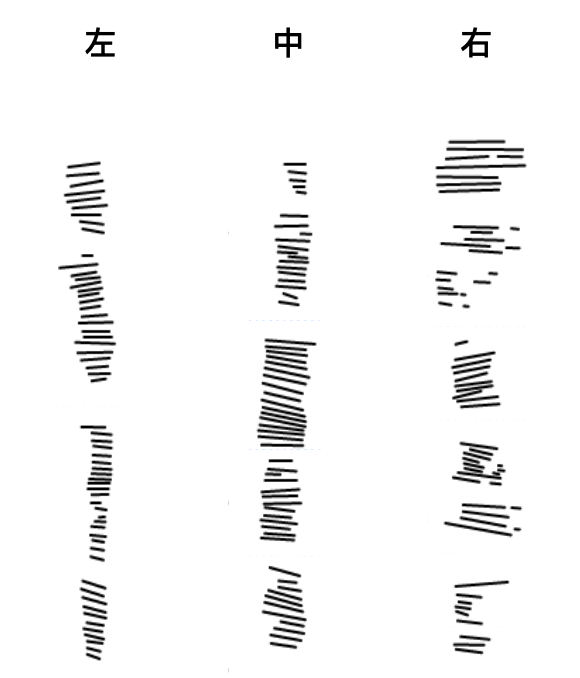
\includegraphics{images/01_03-isango-carved-bone}}
\caption{出土在刚果的 Isango 骨上的刻痕}\label{fig:isango}
\end{figure}

\section{有限性}

几乎可以肯定,当刻痕开始被人类熟练运用,其后不久的某一个时刻,一定有某个人会突然意识到:理论上,刻痕可以无穷无尽的排列下去。
如果历史真的这么展开,这会是人类第一次开始思考无穷的概念。这假想的时刻也将非常可能是“数”作为一个系统第一次登上历史舞台。

\section{一进数制的建立}
